% \begin{savequote}[8cm]
% Alles Gescheite ist schon gedacht worden.\\
% Man muss nur versuchen, es noch einmal zu denken.

% All intelligent thoughts have already been thought;\\
% what is necessary is only to try to think them again.
%   \qauthor{--- Johann Wolfgang von Goethe \cite{von_goethe_wilhelm_1829}}
% \end{savequote}



%\minitoc

%\section{Introduction}



% We define the probability density function (pdf) for a normally distributed random variable $x$ as:

% \begin{equation}
%     f(x; \mu, \sigma^2 ) = \frac{1}{\sigma \sqrt{2 \pi}} \exp{\Bigg[ - \frac{( x - \mu )^2}{2 \sigma^2} \Bigg] }  \tag{$-\infty < x < \infty, -\infty < \mu < \infty, \sigma > 0$}
% \end{equation}
% Here $\mu$ represents the mean, $\sigma^2$ the variance and $\sigma$ the standard deviation of the normal distribution $f(x)$ \cite{patel1996handbook}.
% If we describe $n$ normally distributed random variables, we do this with a multivariate Gaussian:
% \begin{equation}
%     \mathbf{x} = \begin{bmatrix}
%            x_{1} \\
%            \vdots \\ 
%            x_{n}
%          \end{bmatrix} 
%          \sim 
%          \mathcal{N}\begin{pmatrix} 
%          \begin{bmatrix}
%            \mu_{1} \\
%            \vdots \\ 
%            \mu_{n}
%          \end{bmatrix}
%          ,
%          \bm{\Sigma}
%          \end{pmatrix},
% \end{equation}
% where each normally distributed variable $x_i$ with $i = (1 \cdots n)$ has a mean $\mu_i$ and a variance... .
% The inverse of the variance is the precision matrix $\bm{\Sigma}^{-1} = \bm{Q}$
% \begin{align}
%     \pi( \bm{x} ) &= \pi(x_1) \pi(x_2 | x_1) \cdots \pi(x_n | x_{n-1} ) \\
%     &= \frac{1}{(2 \pi)^{n/2}} |\bm{Q}|^{1/2} \ \, \exp{\Bigg[ - \frac{1}{2} \bm{x}^T \bm{Q} \bm{x} \Bigg]} \\ 
%      &= \frac{1}{(2 \pi)^{n/2}} |\bm{\Sigma}|^{-1/2} \exp{\Bigg[ - \frac{1}{2} \bm{x}^T \bm{\Sigma}^{-1} \bm{x} \Bigg]}
% \end{align}

% \begin{equation}
%     \begin{bmatrix}
%            x_{1} \\
%            x_{2}
%          \end{bmatrix} 
%          \sim 
%          \mathcal{N}\begin{pmatrix} 
%          \begin{bmatrix}
%            \mu_{1} \\
%            \mu_{2}
%          \end{bmatrix}
%          ,
%          \begin{bmatrix}
%              \bm{\Sigma}_{11} & \bm{\Sigma}_{12}\\
%              \bm{\Sigma}_{21} & \bm{\Sigma}_{22}
%          \end{bmatrix}
%          \end{pmatrix}
% \end{equation}

% \begin{equation}
%     \begin{bmatrix}
%            x_{1} \\
%            x_{2}
%          \end{bmatrix} 
%          \sim 
%          \mathcal{N}\begin{pmatrix} 
%          \begin{bmatrix}
%            \mu_{1} \\
%            \mu_{2}
%          \end{bmatrix}
%          ,
%         \bm{Q}^{-1}
%          \end{pmatrix}
% \end{equation}

% \begin{align}
% \ln{\pi(\bm{x|y})} =& \ln{\pi( \bm{x} ) } + \ln{ \pi( \bm{y} | \bm{x} ) } \\
% =& - \frac{1}{2} (\bm{x} - \bm{\mu} )^T \bm{Q_x} (\bm{x} - \bm{\mu} ) - \frac{1}{2} (\bm{y} - \bm{Ax} )^T \bm{Q_x} (\bm{y} - \bm{Ax} )    \\
% =& - \frac{1}{2} \bigg[ \bm{x}^T \big[ \bm{Q_x} + \bm{A}^T \bm{Q_y} \bm{A} \big] \bm{x}  + \bm{x}^T \big[ - \bm{A}^T \bm{Q_y} \big] \bm{y} \\
% &+ \bm{y}^T \big[ - \bm{Q_y A} \big] \bm{x} + \bm{y}^T \big[ \bm{Q_y} \big] \bm{y} - 2 \bm{x}^T \bm{Q_x \mu }  \bigg] + \text{const.}
% \end{align}

% \begin{align}
%     &- \frac{1}{2} \begin{bmatrix}
%         \bm{x}^T \big[ \bm{Q_x} + \bm{A}^T \bm{Q_y} \bm{A} \big]  + \bm{y}^T \big[ - \bm{Q_y A} \big] & \bm{y}^T \big[ \bm{Q_y} \big] + \bm{x}^T \big[ - \bm{A}^T \bm{Q_y} \big] 
%     \end{bmatrix}  \begin{bmatrix}
%         \bm{x} \\ \bm{y}
%     \end{bmatrix} \\
%     =& \begin{bmatrix}
%         \bm{x}^T & \bm{y}^T
%     \end{bmatrix} 
%     \underbrace{\begin{bmatrix}
%         \bm{Q}_x + \bm{F}^T \bm{Q}_y \bm{F} & - \bm{F}^T \bm{Q}_y \\
%         -\bm{Q}_y \bm{F} & \bm{Q}_y
%     \end{bmatrix}}_\text{precision matrix} \begin{bmatrix}
%         \bm{x} \\ \bm{y}
%     \end{bmatrix} 
% \end{align}


% \begin{align}
%     \frac{- 2 \bm{x}^T \bm{Q_x \mu } }{-2} = \begin{bmatrix}
%         \bm{x}^T & 0
%     \end{bmatrix} \begin{bmatrix}
%         \bm{Q_x \mu}\\ 0
%     \end{bmatrix} \\
%     \Rightarrow \bm{\mu} = \bm{Q}^{-1} =  \begin{bmatrix}
%         \bm{Q_x \mu}\\ 0
%     \end{bmatrix}
% \end{align}
% \begin{equation}
%     \bm{Q} = \begin{bmatrix}
%         \bm{Q}_x + \bm{F}^T \bm{Q}_y \bm{F} & - \bm{F}^T \bm{Q}_y \\
%         -\bm{Q}_y \bm{F} & \bm{Q}_y
%     \end{bmatrix}
% \end{equation}









% \begin{subequations}
% \begin{align}
%     \bm{x|y, \theta} &\sim \mathcal{N}(\bm{F x}, \bm{Q_y}(\bm{\theta})) \quad \, \text{(likelihood)}\\
%     \bm{x| \theta} &\sim \mathcal{N}(\bm{\mu}, \bm{Q_x}(\bm{\theta})) \qquad \text{(prior)} \\
%     \bm{\theta} &\sim \pi(\bm{\theta}) \qquad \qquad \qquad \! \text{(hyperprior)}
% \end{align}
% \end{subequations}


% % \cite{simpson2012think}



% %\section{Gaussian Markov Random Fields}
% specify locally
% model globally
% set of RV

\chapter{\label{ch:2-litreview}Background}
This chapter provides the background knowledge for the applied methods.
We try to carefully guide the reader through the various topics so that we build a base to understand the used methodology.
Firstly, we discuss Markov Random Fields and their key properties to describe spatially connected variables in Section \ref{subsec:MRF}.
In Section \ref{subsec:NormDist} we introduce the normal distribution to describe the random variables in such a field.
By specifying the local connections in Section \ref{subsec:SpatialDepend} we globally observe a Gaussian Markov Random Field (GMRF).
Next, in Section \ref{sec:Bayesian} we relate the variables in the GMRF to a measurement process through a Bayesian Model.
Given the measurement, we try to find the most likely variables through a Markov chain, as described in Section \ref{subsec:Markov}.
Constructing this Markov chain we present the Metropolis-Hastings algorithm in Section \ref{subsec:MetroHast}, followed by the Marginal and then conditional sampler in Section \ref{subsec:MTC} and the adaptive Metropolis-Hastings algorithm in Section \ref{subsec:GOMOS}. 



\section{Gaussian Markov Random Field}
In this section, we guide the reader through the basic principles of Gaussian Markov Random Fields (GMRF).
We discuss some of the key properties of GMRFs and how to set up such a spatial field.
The discussed topics are strongly related to our specific application and for further reading, we refer to the books \cite{rue2005gaussian, higdon2006primer}.

\subsection{Markov Random Field}
\label{subsec:MRF}
A Markov Random Field (MRF) is based on a graphical model describing spatial dependencies of $n$ nodes, also described as vertices.
We label each node with an integer $i$ and attach a spatial position $s^{(i)}$ and a random variable $x^{(i)}$, where $i = 1, \dots, n$.
On a set of all vertices $\mathcal{V}$ we define an undirected graph $\mathcal{G}(\mathcal{V},\mathcal{E})$ with a set of edges $\mathcal{E}$.
If an edge describes spatial dependencies of a pair of different nodes $i$ and $j$ then we write $i \sim j$, where $(i,j) \in \mathcal{E}$, with no preferred direction.
We limit interactions to pair-wise only.

For a subset of nodes $A = \mathcal{V}^A \subset \mathcal{V}$, we can define a subgraph $\mathcal{G}^\mathcal{A}(\mathcal{V}^A,\mathcal{E}^A)$ , including edges  $\mathcal{E}^A = \{ (i,j)\in \mathcal{E} \text{ and } i,j \in \mathcal{V}^A \text{ and } i \neq j \}$.
A discrete example is illustrated in Figure \ref{fig:MRFGRAPH}.


Through the Markov properties of such a field, a single node $i$ is conditionally dependent on its neighbors $\partial i = \{ j : (i,j) \in \mathcal{E} \text{ and } j \neq i   \}$ only.
We denote $-A = \mathcal{V} - A $ to all nodes not in $A$ but part of $\mathcal{V}$.
Similarly, we can extend this to a subset $A \in \mathcal{V}$ where the neighborhood $\partial A = \{ j : (i,j) \in \mathcal{E} \text{ and } j \notin A\}$ is all nodes $j \in -A$ sharing an edge to a node $ i \in \mathcal{V}^A$.
Conditioned on all its neighbours $\mathcal{V}^A$ is independent of all other notes $\pi(\bm{x}^{(A)}|\bm{x}^{(-A)}) = \pi(\bm{x}^{(A)}|\bm{x}^{(\partial A)}) $.
Here $\pi(\cdot)$ denotes the probability density for its argument.
Intuitively we interpret $\bm{Q}$ in terms of conditional dependencies and $\bm{\Sigma}$ marginally, which reduces distribution to maximal $n$ dimensional.

\subsection{Multivariate Normal Distribution}
\label{subsec:NormDist}
In our case, we specifically choose a probability density that distributes each random variable $x^{(i)}$ normally and denote this with $x^{(i)} \sim \mathcal{N}(\mu^{(i)}, \sigma)$.
Here $\mu_i = \text{E}(x^{(i)})$ is the mean of $x^{(i)}$ and $\sigma^2 = \text{Var}(x^{(i)}) $ is the variance of any $x^{(i)}$.

Constructing a Gaussian Markov Random Field (GMRF), we introduce a normal probability density function $\pi$ for a single node $x_i$, with mean $\mu$ and variance $\sigma^2$.
%\mccorrect{$\pi() oder \, f $ and multivariate, change to $\pi(x_i)$}
\begin{equation}
    \pi(x^{(i)}) = \frac{1}{\sqrt{2 \pi \sigma^2}} \exp{\Bigg[ - \frac{( x^{(i)} - \mu^{(i)} )^2}{2 \sigma^2} \Bigg] }  %\tag{$-\infty < x < \infty, -\infty < \mu < \infty, \sigma > 0$}
\end{equation}
To describe the values of all nodes in a GMRF we introduce a multivariate Gaussian
\begin{equation}
    \bm{x} = \begin{bmatrix}
           x^{(1)} \\
           \vdots \\ 
           x^{(n)}
         \end{bmatrix} 
         \sim 
         \mathcal{N}\begin{pmatrix} 
         \begin{bmatrix}
           \mu^{(1)} \\
           \vdots \\ 
           \mu^{(n)}
         \end{bmatrix}
         ,
         \bm{\Sigma}
         \end{pmatrix},
\end{equation}
with a covariance matrix $\mathbf{\Sigma} = \bm{Q}^{-1}$, which is the inverse of the precision-matrix.
As we deal with an undirected Markov field, $\bm{Q}$ is a symmetric positive-definite matrix and sparse.
Hence, we can efficiently decompose $\bm{Q} = \mathbf{L} \mathbf{L}^T$ into its Cholesky triangle $\mathbf{L}$, which is a lower triangular matrix.
Within this precision matrix, we can define the interactions and correlations between the different nodes of our GMRF.


When constructing a GMRF the precision matrix $\bm{Q}$ as well as its inverse $\bm{\Sigma}$ does a play key role.
If the GMRF is fully connected them $\bm{Q}$ is completely dense, we aim to construct a GMRF so that the precision matrix is sparse.
The off diagonal non-zero entries of $\bm{Q}$ provide information about conditional correlations $\text{Corr}(x^{(i)}, x^{(j)} | \bm{x}^{(-ij)}) = Q_{ij} / \sqrt{Q_{ii} Q_{jj}}$.
Where as the off diagnopal entries of $\bm{\Sigma}$ give information about marginal correlations $\text{Corr}(x^{(i)}, x^{(j)}) = \Sigma_{ij} / \sqrt{\Sigma_{ii} \Sigma_{jj}}$.
The diagonal entries provide marginal variances $\text{Var}(x^{(i)}) = \Sigma_{ii}$ and conditional precision $\text{Prec}(x^{(i)},x^{(j)} | \bm{x}^{(-ij)}) =  Q_{ii}$.


%+++++++++++++++++++++++++++++++++++++++++++++++++++++++++++++++++++++++++++++++++++
\subsection{Conditional distribution through Spatial Dependencies}
\label{subsec:SpatialDepend}
\label{subsec:precQ}
\begin{figure}[thb!]
    \centering
        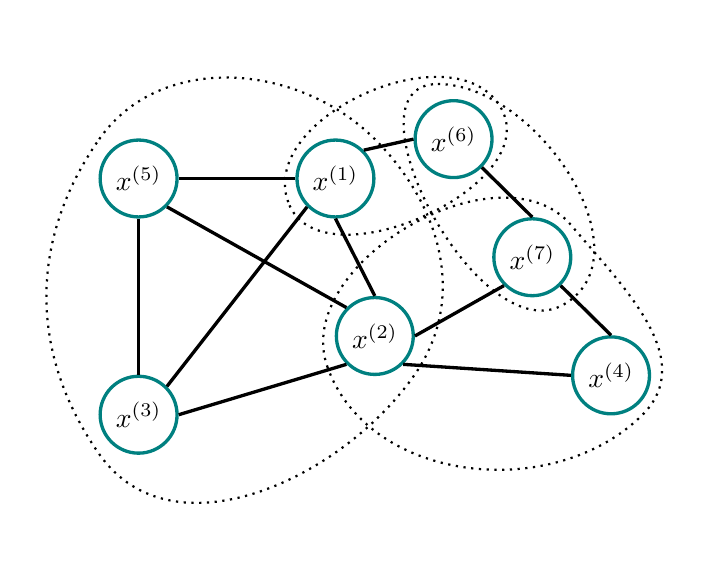
\begin{tikzpicture}[
roundnode/.style={circle, draw=green!50!blue, fill=green!60!blue, very thick, minimum size=7mm},
roundnode2/.style={circle, draw=green!50!blue, very thick, minimum size=9mm},
%squarednode/.style={rectangle, draw=red!60, fill=red!5, very thick, minimum size=5mm},
]
%Nodes
\node[roundnode2] at (2.5,4) (1)     {$x^{(1)}$};
\node[roundnode2] at (3,2) (2)     {$x^{(2)}$};
\node[roundnode2] at (0,1) (3)     {$x^{(3)}$};
\node[roundnode2] at (6,1.5) (4)     {$x^{(4)}$};
\node[roundnode2] at (0,4) (5)     {$x^{(5)}$};
\node[roundnode2] at (4,4.5) (6)     {$x^{(6)}$};
%\node[roundnode] at (1,2.5) (7)     {7};
\node[roundnode2] at (5,3) (8)     {$x^{(7)}$};
%Lines
\draw[-, very thick] (1.west) -- (5.east);
\draw[-, very thick] (1.north east) -- (6.west);
\draw[-, very thick] (1.south) -- (2.north);
%\draw[-, very thick] (1.south west) -- (7.north east);
%\draw[-, very thick] (1.south east) -- (8.west);
\draw[-, very thick] (8.south west) -- (2.east);
\draw[-, very thick] (8.south east) -- (4.north);
\draw[-, very thick] (4.west) -- (2.south east);
\draw[-, very thick] (3.east) -- (2.south west);
%\draw[-, very thick] (3.north east) -- (7.south west);
%\draw[-, very thick] (2.west) -- (7.east);
\draw[-, very thick] (3.north) -- (5.south);
\draw[-, very thick] (6.south east) -- (8.north);
\draw[-, very thick] (5.south east) -- (2.north west);
\draw[-, very thick] (1.south west) -- (3.north east);
%\draw[-, very thick] (5.south east) -- (7.north west);
% \draw[dotted, very thick] (1.north) -- (1a.south);
% \draw[dotted, very thick] (3.north) -- (3a.south);
% \draw[dotted, very thick] (2.north) -- (2a.south);
% \draw[dotted, very thick] (4.north) -- (4a.south);
%Cliques and (-1,0)
%5-1-2-3-5
\draw[dotted, thick] (-0.5,4.5)
    to[out=55,in=135] (3,4.5)
    to[out=315,in=55](3.5,1.5)
    to[out=-125,in=-55] (-0.5,0.5)
    to[out=125,in=-125] (-0.5,4.5);
%6-7-6
\draw[dotted, thick] (3.8,5.2)
    to[out=0,in=30] (5.4,2.4)
    to[out=-150,in=180] (3.8,5.2);
%2-7-4-2
\draw[dotted, thick] (2.4,1.6)
    to[out=110,in=130](5.5,3.4)
    to[out=-50,in=45] (6.4,1)
    to[out=-135,in=-70] (2.4,1.6);
%1-6-1
\draw[dotted, thick] (1.9,3.7)
    to[out=110,in=120](4.6,4.9)
    to[out=-60,in=-70] (1.9,3.7);
\end{tikzpicture}
    \caption[Undirected Random Field of seven nodes including maximum cliques.]{\textbf{Undirected Random Field of seven nodes including maximum cliques.} The random field displayed here can be described with a Graph $\mathcal{G}$. Where $\mathcal{V}$ are all nodes seen in the figure and $\mathcal{E}$ are the edges drawn with a line between nodes. We draw dotted lines around the set of maximum cliques, which are not a full subset of any other clique. Maximum cliques are a set of fully connected nodes with common neighbors. A neighborhood is defined through an edge between two nodes, such as $\{ x^{(1)}, x^{(6)}\} \in \mathcal{E}$. Here $ \{ \{ x^{(1)}, x^{(6)}\}, \{ x^{(1)}, x^{(3)}, x^{(4)}, x^{(5)} \}, \{ x^{(6)}, x^{(7)} \}, \{ x^{(2)}, x^{(4)}, x^{(7)} \} \}$ form the set of maximum cliques.
    On a set of maximum cliques, we can define an energy function, Gibbs distribution or use the \mccorrect{conditional auto regressive model} to define spatial dependencies.
    The precision matrix $\bm{Q}$ represents those spatial dependencies weighted by the hyper parameter $\bm{\theta}$.}
    \label{fig:MRFGRAPH}
\end{figure}

In this subsection, we present the Conditional Auto Regressive (CAR) model and the Gibbs field to define a graph $\mathcal{G}(\mathcal{V},\mathcal{E})$ and the corresponding precision matrix $\bm{Q}$.
For curious readers we recommend the book \cite{bremaud2013markov}.

The CAR method can include neighbouring nodes of numerous orders.
We define the entries of the precision matrix as follows:
\begin{equation}
      Q_{ij} = \begin{cases}
          \kappa_i & i = j \\
        \kappa_i \beta_{ij} & i \neq j
      \end{cases},
  \end{equation}
where $\beta_{ij} = 0 $, if $x^{(i)}$ and $x^{(j)}$ are conditionally independent, and $\kappa_i > 0$ to ensure positive-definiteness of $\bm{Q}$ for all $i = 1, \dots, n$.
The full conditionals are normally distributed
\begin{equation}
    x^{(i)} | x^{(-i)} = x^{(i)} | \partial x^{(i )} \sim \mathcal{N} \big( \underbrace{\sum_{j:j\neq i} \beta_{ij} x^{(j)}}_{\text{mean}}  \, , \, \underbrace{\kappa_i^{-1}}_{\text{variance}} \big)
\end{equation}
and depend only on neighbouring nodes $\partial x^{(i )}$ having an edge to $x^{(i)}$.
We can then write the probability density over all nodes $\bm{x}$ including their means $\bm{\mu}$ as follows:
\begin{align}
    \pi( \bm{x} ) %&= \pi(x_1) \pi(x_2 | x_1) \cdots \pi(x_N | x_{N-1} ) \\
    &= \frac{1}{(2 \pi)^{n/2}} \sqrt{\det(\bm{Q})} \ \, \exp{\Bigg[ - \frac{1}{2} ( \bm{x} - \bm{\mu} )^T \bm{Q} (\bm{x} - \bm{\mu}) \Bigg]} \\ 
     &= \frac{1}{(2 \pi)^{n/2}} |\bm{\Sigma}|^{-1/2} \exp{\Bigg[ - \frac{1}{2} ( \bm{x} - \bm{\mu} )^T \bm{\Sigma}^{-1} ( \bm{x} - \bm{\mu} ) \Bigg]} \, .
\end{align}

Alternatively, we can describe a set of nodes through a Gibbs field, where we define a clique $c \in \mathcal{C}$ as a set of fully connected nodes.
In a clique each node $j \in c$ has mutual neighbours to any other node $i \neq j \in c$. 
If for any node $j \notin c$ and $j \in \mathcal{V}$, the union of $j \cup c$ is not a clique then we call $\tilde{c} \in \mathcal{C}$ a maximal clique.
We conclude that maximal cliques are not a complete subset of another clique.
%\mccorrect{double check if concept of cliques \textbf{and} maximum cliques has to be explained}
The positive clique-potential $\phi_{\tilde{c}}(\tilde{c})$ describes the interactions of all nodes within a clique.
The sum over all maximum clique-potentials is often described as the Energy:
\begin{equation}
    E = \sum_{\tilde{c} \in \mathcal{C}} \phi_{\tilde{c}}(x^{(i)} : x^{(i)} \in c).
\end{equation}
We normalize the Gibbs distribution $\pi(\bm{x})$ of a random field with a normalization constant $Z$.
\begin{align}
    \pi(\bm{x}) &= \frac{1}{Z} \exp{ \Big[ -\sum_{\tilde{c}\in \mathcal{C}} \phi_{\tilde{c}}(x^{(i)} : x^{(i)} \in \tilde{c}) \Big] } \\
    &Z = \sum_{i \in \mathcal{V}} \prod_{\tilde{c} \in \mathcal{C}} \exp{ \Big[ - \phi_{\tilde{c}} (x^{(i)}: x^{(i)} \in \tilde{c}) \Big] } 
\end{align}


The Hammersley-Clifford theorem states that if we describe any Random Field through a Gibbs distribution over maximum cliques then we deal with a MRF.
First proven by Julien Besag we can show that conditional joint distribution is expressed as
\begin{align}
\pi(x^{(i)} | \partial x^{(i)}) &= \frac{1}{Z} \exp{\big[  -\sum_{\tilde{c} \in \mathcal{C}} \phi_{\tilde{c}}(x^{(i)},x^{(j)} : i,j \in \tilde{c} \text{ and } i \neq j) \big]}\\
     &Z = \sum_{i \in \mathcal{V}} \prod_{\tilde{c} \in \mathcal{C}} \exp{ \Big[ - \phi_{\tilde{c}} (x^{(i)},x^{(j)}: i,j \in \tilde{c} \text{ and } i \neq j) \Big] }
\end{align}
and can be found in \cite{besag1974spatial}.
% To actually model an MRF based on a Gibbs field we set up one clique potential and connect the neighbouring sites in a 2D lattice
% \begin{equation}
%     \phi_c(x_i,x_j) = \begin{bmatrix}
%                         x_{i} & x_{j}
%                      \end{bmatrix}  
%                      \underbrace{\begin{bmatrix}
%                         w_{ij} & -w_{ij} \\
%                         -w_{ji} & w_{jj}
%                      \end{bmatrix}}_{\mathbf{W}} 
%                      \begin{bmatrix}
%                         x_{i} \\ x_{j}
%                      \end{bmatrix}  
%                      % \begin{bmatrix}
%                      %    e^{w_{ij}} & e^{-w_{ij}} \\
%                      %    e^{-w_{ji}} & e^{w_{jj}}
%                      % \end{bmatrix} 
% \end{equation}
% if not neighbours the $w_{ij} = 0$, assume symmetrie in within the weight matrix $\mathbf{W}$.
% \begin{align}
%     \ln{ \pi(x_i| \partial x_i) } \propto - \frac{1}{2} \mathbf{x}^T \mathbf{W} \mathbf{x} + \mathbf{b}^T \mathbf{y} \\
%     \pi(x_i| \partial x_i) \propto \exp{\Bigg[- \frac{1}{2} (\mathbf{y} - \mu)^T \mathbf{\Sigma}^{-1} (\mathbf{y} - \mu)  \Bigg]}
% \end{align}
The potential $\phi_{\tilde{c}}$ can describe the interactions between different nodes of a Gaussian Gibbs field if set accordingly, which leads to the precision-matrix $\bm{Q}$ for a Gaussian Markov Random Field (GMRF).
%\mccorrect{For example with specific $\phi_c$/$\bm{Q}$ see application/appendix}





%define nieghbourhood struicture
%\begin{itemize}
  % \item CAR
  
  % % symmetry: $k_i \beta_{ji} = k_j \beta_{ij}$ for all $i \neq j$\\
  % % positive definiteness $\kappa_i > 0$ for all $i = 1, \dots, n$\\
  % % if $Q_{i,j} = 0$ $x_j$ and $x_i$ are conditionally independent\\
  % % if $Q_{i,j} \neq 0$, $\beta_{i,j} \neq 0$ $i \neq j$ then $x_j$ and $x_i $ are conditional dependent, neighbours, have an edge\\
  % % conditional $x_i | x_{-i} = x_i | x_{\partial i } \sim \mathcal{N}(\underbrace{\sum_{j:j\neq i} \beta_{i,j} x_j}_{\text{mean}}  \, , \, \underbrace{\kappa_i^{-1}}_{\text{variance}} )$\\
  % % choose $\beta and \kappa $
  
  % \item cliques

  
  %\item specify Q directly
  % \item Gibbs Distribution

  %  The Markov property describes conditional dependence of image signals within a local neighbourhood system, which is proved to be useful in capturing and modelling usually highly localised and coherent texture features. Another appealing property of an MRF is that, by the Hammersley-Clifford theorem [42], an MRF can be characterised by a global Gibbs distribution. \\
  %  define cliques\\
  %  define maximum cliques\\
  %  maximum clique potential\\
  %  \begin{equation}
  %      E() = \sum_{c_i \in \mathcal{C}} \Phi(x_j : j \in c_i)
  %  \end{equation}
  %  \begin{equation}
  %      Pr() = \frac{1}{Z} \exp{ \{  - E  \} }
  %  \end{equation}
  %  normalisation\\
  %  \begin{equation}
  %      \pi(x_i | \partial x_i) = \frac{1}{Z_i} \exp{}
  %  \end{equation}
   
  %  Hammersley-Clifford Theorem, besag\\
  %  MRF condintional \\
  %  choose function $\phi$
   
%\end{itemize}

\section{linear-Gaussian hierarchical Bayesian model}
\label{sec:Bayesian}
Bayesian hierarchical models are a very helpful tool to describe a measurement process through different layers of complexity.
It allows us to backtrack from our observations to the source of the measurement in a \mccorrect{very precise/simplified} way.
Here we closely follow the terminology of \cite{fox2016fast, simpson2012think}


\begin{figure}[thb!]
    \centering
    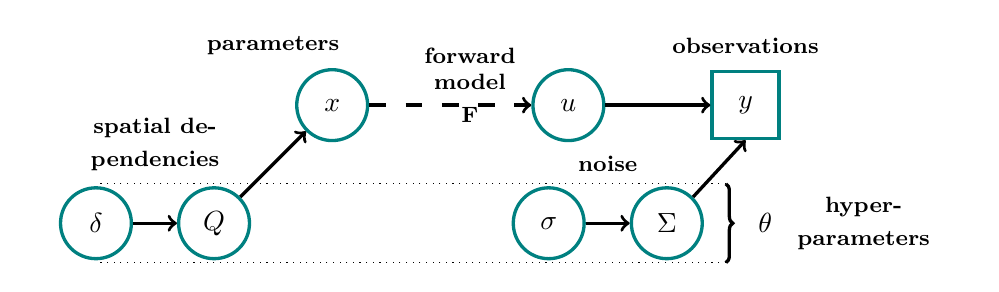
\begin{tikzpicture}[
roundnode/.style={circle, draw=green!50!blue, fill=green!60!blue, very thick, minimum size=7mm},
roundnode2/.style={circle, draw=green!50!blue, very thick, minimum size=9mm},
rectnode/.style={rectangle, draw=green!50!blue, very thick, minimum size=8.5mm},
mydotted/.style = {dash pattern=on 6.1pt off 7pt},
%squarednode/.style={rectangle, draw=red!60, fill=red!5, very thick, minimum size=5mm},
]
%Nodes
%\node[roundnode] at (0,0) (1)     {1};
\node[roundnode2] at (-1.5,-1.5) (H1)     {$\bm{Q}$};
\node[roundnode2] at (0,0) (1)     {$\bm{x}$};
\node[roundnode2] at (3,0) (2)    {$\bm{u}$};
\node[rectnode] at (5.25,0) (3)    {$\bm{y}$};
\node[roundnode2] at (4.25,-1.5) (H3)    {$\bm{\Sigma}$};
\node[roundnode2] at (2.75,-1.5) (HN)    {$\sigma$};
\node[roundnode2] at (-3,-1.5) (HP)    {$\delta$};
%text
\draw (1.75,0.25) node[align=center, text width=1.5cm] {\footnotesize \textbf{forward model \\ F}};
\draw (6.75,-1.5) node[align=center, text width=2.5cm] {\footnotesize \textbf{hyper\-parameters}};
\draw (5.5,-1.5) node[align=center, text width=0.5cm] { $\bm{\theta}$};
\draw (5.25,0.75) node[align=center, text width=3cm] {\footnotesize \textbf{observations}};
\draw (-0.75,0.75) node[align=center, text width=3cm] {\footnotesize \textbf{parameters}};
\draw (-2.25,-0.5) node[align=center, text width=3cm] {\footnotesize \textbf{spatial dependencies}};
%\draw (-1.4,-2.3) node[align=center, text width=3cm] {\footnotesize \textbf{hyper-prior}};
\draw (3.5,-0.75) node[align=center, text width=3cm] {\footnotesize \textbf{noise}};
% Calligraphic brace
\draw[very thick, decorate,decoration = {brace}] (5,-1) --  (5,-2);

%Lines
\draw[->, very thick] (HN.east) -- (H3.west);
\draw[->, very thick] (HP.east) -- (H1.west);
\draw[->, very thick] (H1.north east) -- (1.south west);
\draw[->, mydotted, very thick] (1.east) -- (2.west);
\draw[->, very thick] (2.east) -- (3.west);
\draw[->, very thick] (H3.north east) -- (3.south);
\draw[dotted] (5,-1) -- (-3,-1);
\draw[dotted] (5,-2) -- (-3,-2);
\end{tikzpicture}
    \caption[A hierarchical Bayesian model describes how we model a physical process to observe data.]{\textbf{A Bayesian hierarchical model describes how we model a physical process to observe data.} Through a forward model we describe a physical process depending on some parameters $\bm{x}$.
    The spatial dependencies of those parameters $\bm{x}$ are described through the hyper-parameters $\bm{\theta} = (\delta, \sigma)$.
    The precision matrix $\bm{Q}$ is defined according to our \changelinkcolor{black}\hyperref[subsec:MRF]{Markov Random field} and the amount of interaction between certain nodes is described by $\delta$.
    The forward map $\bm{F}$ models a physical process and maps the parameters $\bm{x}$ to a space of all measurable $\bm{u}$.
    From this space $\bm{u}$, we observe some data including some random noise $\gamma$ with variance $\bm{\Sigma}(\gamma)$.
    A Bayesian framework allows us to find the most likely parameters and hyper-parameters $\bm{x}, \bm{\theta}| \bm{y}$ given our measurement .}
    \label{fig:BAYHIER}
\end{figure}

Usually, a measurement device delivers some data $\bm{y}$ including some noise $\sigma$ and we like to model the observation to quantify some unknown parameters $\bm{x}$ and their unknown spatial dependencies.
%Given the observed data vector $\bm{y}$ we would like to quantify the unknown parameter vector $\bm{x}$, including the uncertainty of $\bm{x}$, and the hyper-parameter vector $\bm{\theta}$. corresponding to the hyper-prior $\pi ( \bm{\theta} ) $ 
%As discussed in the subsection, we set up a graphical model to describe spatial dependencies within our parameter field, as seen in figure \ref{fig:MRFGRAPH} $\bm{x|\bm{\theta}}$.
Through the precision matrix $\bm{Q}(\delta)$, we define neighborhoods and weight pair-wise interactions of parameters $x^{(j)} \text{ and } x^{(i)}$ according to a hyper-prior distribution $\pi ( \delta ) $ in (\ref{eq:hyper}).
The inverse of the precision matrix $\bm{Q}( \delta ) $ is the variance of the prior distribution $\pi(\bm{x} |  \bm{Q}^{-1}( \delta ) )$ in (\ref{eq:prior}), and usually sparse.
Based on this graphical model we map $\bm{x}$ through a forward model $\bm{F}$ \mccorrect{Dimensions} to space of all measurables $\bm{u}$.
%Given a forward model $\bm{F}$, which typically describes a physical process, we map the parameters to a so-called space of all measurable $\bm{u}$.
Next, we observe some data $\bm{y} = \bm{F} \bm{x} + \gamma$ and add some unknown normally distributed random noise $\eta$ with variance $\bm{\Sigma}(\gamma)$.
We assume that this noise vector is independent and identically distributed (i.i.d.).
The likelihood function $\pi( \bm{y} | \bm{x, \theta} )$ in (\ref{eq:likeli}) describes how likely/realistic the observations $\bm{y}$ are.
In our specific case, we choose a linear forward model and a Gaussian prior, so that our likelihood function and posterior distribution in (\ref{eq:post}) are normally distributed as well.
In doing so we can find an analytic expression for the uncertainty of the posterior and see that it is depending on both the prior and the likelihood distribution, for more details we refer to the Appendix \ref{ap:bayesian}.

In Equations (\ref{eq:prior}) - (\ref{eq:hyper}), we summarize a hierarchical Bayesian model in a generalized form, with the hyper-parameter $\bm{\theta} = (\delta, \gamma)$.
Note that in this case we define two hyper-parameters, but we can increase the dimensions of $\theta$ to an arbitrary number suitable to describe the underlying physical process sufficiently.
\begin{subequations}
\begin{align}
     \label{eq:likeli}
    \bm{y|x, \theta} &\sim \mathcal{N}(\bm{F x}, \bm{\Sigma}(\bm{\theta}) ) \qquad \quad   \, \text{(likelihood)}\\
    \label{eq:prior}
    \bm{x| \theta} &\sim \mathcal{N}(\bm{\mu}, \bm{Q}^{-1}(\bm{\theta}) ) \qquad \qquad  \quad \! \! \! \text{(prior)} \\
    \label{eq:hyper}
    \bm{\theta} &\sim \pi(\bm{\theta}) \qquad \qquad \qquad \qquad \quad \; \, \text{(hyper-prior)}
 \end{align}
 The posterior has the following from
 \begin{align}
     \label{eq:post}
    \bm{x , \theta|y} &\sim \mathcal{N}( \mu_{\bm{x , \theta|y} } , ( \bm{Q} + \bm{F}^T\bm{\Sigma}^{-1}\bm{F} )^{-1} ) \quad  \text{(posterior)}
\end{align}
\end{subequations}
with the mean $\mu_{\bm{x , \theta|y} } = \bm{\mu} + (\bm{Q} + \bm{F}^T \bm{\Sigma}^{-1} \bm{F})^{-1} \bm{F}^T \, \bm{\Sigma}^{-1} (\bm{y} - \bm{F \mu})$. 


Using \mccorrect{Bayes} theorem we can find an expression for the posterior distribution $\pi (\bm{x} , \bm{\theta} | \bm{y})$ for the parameters $\bm{x}$ and the hyper-parameters $\bm{\theta}$ given the observed data $\bm{y}$.
\begin{align}
    \pi (\bm{x} , \bm{\theta} | \bm{y}) &= \frac{\pi( \bm{y} | \bm{x}, \bm{\theta} ) \, \pi(\bm{x},  \bm{\theta}) }{\pi(\bm{y})}
    %& \propto \pi( \bm{y} | \bm{x}, \bm{\theta} ) \, \pi(\bm{x} |  \bm{\theta}) \pi( \bm{\theta} )
\end{align}

%We obtain a posterior probability distribution proportional to the distribution in our Bayesian hierarchical model, see equations \ref{eq:hyper} - \ref{eq:likeli}.
If we like to compute the posterior distribution we have to compute the normalization constant $\pi(\bm{y})$, where we marginalize out $\bm{x}$ and $\bm{\theta}$ :
\begin{equation}
    \pi(\bm{y}) = \int \int \pi(\bm{y}, \bm{x}, \bm{\theta}) \diff \bm{x} \diff \bm{\theta} \, ,
\end{equation}
which can yield a extensive computation.
% Usually this is computationally too expensive, but if we assume that the normalization constant $\pi(\bm{y}) $ is finite and non zero
% we obtain a posterior proportional to the distribution in our hierarchical model:
% \begin{align}
%     \pi (\bm{x} , \bm{\theta} | \bm{y}) \propto \pi( \bm{y} | \bm{x}, \bm{\theta} ) \, \pi(\bm{x} |  \bm{\theta}) \pi( \bm{\theta} ) \, .
% \end{align}
Using the posterior density we can find the expected value of any function $h(\bm{x})$ though an average of the function weighted by the probability density distribution $\pi (\bm{x} , \bm{\theta} | \bm{y})$.
\begin{equation}
    \text{E}_{\bm{x},\bm{\theta}|\bm{y}} [h(\bm{x})] = \int \int h(\bm{x}) \pi( \bm{x}, \bm{\theta} | \bm{y}) \diff \bm{x} \diff \bm{\theta} 
\end{equation}

\mccorrect{Taking a look at the posterior we can see that $\pi(\bm{x}, \bm{\theta} | \bm{y})$.. and see that to solve this might be very tidious, where as the ratio is much easier...}
\begin{align}
    \pi(\bm{x}, \bm{\theta} | \bm{y}) &\propto  \pi(\bm{y}|  \bm{x}, \bm{\theta} )  \pi(\bm{x}|  \bm{\theta} )  \pi(\bm{\theta} ) \\
    &= \frac{  \pi(\bm{\theta})}{\sqrt{ \det( \bm{\Sigma}) \,  \det( \bm{Q} )^{-1}  } } \exp{ \Bigg[  \frac{(\bm{F \mu} - \bm{y})^T  (\bm{F \mu} - \bm{y})}{\bm{\Sigma}} + \frac{(\bm{\mu} - \bm{x})^T  (\bm{\mu} - \bm{x}) }{\bm{Q}^{-1}}\Bigg] }
\end{align}

If we set $h(\bm{x}) = \bm{x}$ we get the mean of the parameter $\bm{x}$ or the posterior covariance if $h(\bm{x}) = (\bm{x} - \text{E}_{\bm{x},\bm{\theta}|\bm{y}} [\bm{x}]) (\bm{x} - \text{E}_{\bm{x},\bm{\theta}|\bm{y}} [\bm{x}] )^T $.
Computing that is very expensive and usually not feasible as the parameters can too many different values, depending on the range and complexity of the problem.
Instead, we can explore the parameter space for a few (e.g. $10^4$) discrete values and use the Monte-Carlo method to approximate the integral.
%and compare in between the generated samples of the posterior.
%One way of moving and picking values in our parameter space is through a so-called Markov-chain Monte Carlo (MCMC) algorithm.


\subsection{Monte-Carlo Method Integration}
The Monte-Carlo method was first developed in Los Alamos, United States of America, just after the II world war to simulate the flight path of neutrons.
Later in 1949, N. Metropolis and S. Ulam formulated their ideas already suggesting to use 'Markoff' chains in Monte Carlo simulations to approximate continuous functions \cite{metropolis1949monte}.
%Using random values .
For more details on the fundamental theorems we use in this work, we refer to the books \cite{hammersley1964general, whitlock1986monte}

Using the Monte-Carlo method we can approximate the expected value of any function $h(\bm{x})$ by the sample mean:
\begin{equation}
\label{eq:sampMean}
    \text{E}_{\bm{x},\bm{\theta}|\bm{y}} [h(\bm{x})] =  \int \int   \bm{x} \,  \pi(\bm{x}, \bm{\theta} | \bm{y} ) \, \text{d} \bm{x}  \, \text{d} \bm{\theta} \approx \frac{1}{N +1} \sum_{i=0}^{N} \bm{x}_{i} \, ,
\end{equation}
where we draw $n$ parameter samples $\bm{x}_{i}$ from the posterior distribution $\pi (\bm{x} , \bm{\theta} | \bm{y})$.
%If we set $h(\bm{x}) = \bm{x}$ we get the mean or the posterior covariance if $h(\bm{x}) = (\bm{x} - \text{E}_{\bm{x},\bm{\theta}|\bm{y}} [\bm{x}]) (\bm{x} - \text{E}_{\bm{x},\bm{\theta}|\bm{y}} [\bm{x}] )^T $.
We can argue with the central limit theorem that if $N \rightarrow \infty$ the sequence of $ \{ \bm{x}_{0}, \dots, \bm{x}_{N} \}$ converges the sample mean and sample variance to the true mean and true covariance of $\pi( \bm{x}, \bm{\theta} | \bm{y})$.
In our case, we know that the posterior is normally distributed and the task now is to draw samples from this distribution to perform such an integration.
The problem is that it is not feasible to compute the posterior distribution due to the size of the parameter space.
Instead, we construct a Markov chain of randomly picked parameters, which converges to the posterior distribution.

\subsection{Markov Chains}
\label{subsec:Markov}
First formulated by Andrey Markov and published in 1906, Markov chains are a very useful statistical tool to describe real-world processes \cite{markov2006extension}. 
In this section, we discuss some of the properties of Markov chains to make sure that we sample from a unique equilibrium distribution, which is in our case the posterior distribution $\pi (\bm{x} , \bm{\theta} | \bm{y})$.
We like to show aperiodicity, irreducibility, and convergence towards a stationary distribution by proofing the detailed balance condition.
If all of these properties hold we call a chain ergodic with a unique equilibrium distribution, e. g. $\pi (\bm{x} , \bm{\theta} | \bm{y})$.
For more detailed information we refer to \cite{fox2010introduction, bremaud2013markov}.

%\mccorrect{ergodic chain convergence guaranteed by the central limit theorem}
%We explore the parameter space of our Bayesian hierarchical model and generate a Markov chain.
%For the sequence of parameter values we calculate the corresponding posterior distribution.
%We require this Markov chain to be ergodic.
%This means that the chain converges to an equilibrium distribution, which is in our case the posterior distribution, and each drawn state is reachable by any other state, meaning the chain is aperiodic.

%Markov
In a finite parameter space $\Omega(\mathcal{X},\mathcal{\theta})$ we draw a sequence of random variables  $ \mathcal{M} = \big \{ \{ \bm{x}_0, \bm{\theta}_0 \} , \{ \bm{x}_1, \bm{\theta}_1 \} , \dots , \{ \bm{x}_N, \bm{\theta}_N \} \big \}$ from distributions $ \pi^{(0)}, \dots , \pi^{(N)}$  .
The Markov condition requires that each transition probability $\text{Pr}(\cdot)$ of a new state $\{ \bm{x}_{N+1}, \bm{\theta}_{N+1} \}$ only depends on the current state $\{ \bm{x}_{N}, \bm{\theta}_{N}\}$:
\begin{align}
    \text{Pr}(\{ \bm{x}_0, \bm{\theta}_0 \} , \{ \bm{x}_1, \bm{\theta}_1 \} , \dots , \{ \bm{x}_N, \bm{\theta}_N \}) &=  \text{Pr}(\{ \bm{x}_{N+1}, \bm{\theta}_{N+1} \}| \{ \bm{x}_N, \bm{\theta}_N \} \, .
\end{align}

%distributions
For reasons of simplicity in terminology we denote the state $\{ \bm{x}_N, \bm{\theta}_N \}$ as vector $(\bm{x}^T_N, \bm{\theta}^T_N )^T = \bm{i}$
The probability for the Markov chain to be in that state $\bm{i}$ after $N$ steps is denoted as $\pi^{(N)}_{\bm{i}} = \text{Pr}( (\bm{x}^T_N, \bm{\theta}^T_N )^T = \bm{i})$.
We arrange the probability distribution of the $N$th step as a row vector representing the probabilities to be in different states $\bm{i},\bm{j} \in \Omega( \mathcal{X}, \mathcal{\theta} )$
\begin{align}
     \pi^{(N)} = \begin{bmatrix}
          \cdots 
           \pi^{(N)}_{\bm{i}} 
          \pi^{(N)}_{\bm{j}} 
          \cdots 
         \end{bmatrix}
\end{align}


%homogenous
A Markov chain $\mathcal{M}$ is homogeneous if the transition probability only depends on the value of the current and proposed state and not on $n$, the position in the chain.
\begin{equation}
    \text{Pr}(\{ \bm{x}_{N+M+1}, \bm{\theta}_{N+M+1} \}| \{ \bm{x}_{N+M}, \bm{\theta}_{N+M} \}) = \text{Pr}(\{ \bm{x}_{N+1}, \bm{\theta}_{N+1} \}| \{ \bm{x}_N, \bm{\theta}_n \} ) \quad \forall M \in \mathbb{Z}
\end{equation}
Then we denote the probability to transition from state $\{ \bm{x}_N, \bm{\theta}_N \} = i$ to $\{ \bm{x}_{N+1}, \bm{\theta}_{N+1} \}= j $ as an element of the transition matrix $\bm{P}$:
\begin{equation}
    P_{\bm{i j}} =  \text{Pr}( ( \bm{x}^T_{N+1}, \bm{\theta}^T_{N+1} )^T = \bm{j}| ( \bm{x}^T_N, \bm{\theta}^T_N )^T  = \bm{i}) 
\end{equation}
This matrix represents the transitions for one step from
%stationary distribution
As we draw more and more states, some of those states are more likely to occur than others.
The Chain will reach an equilibrium distribution $\pi^{(N)} \rightarrow \pi$ as $N \rightarrow \infty$.
We call $\pi$ the stationary distribution for the transition matrix $\bm{P}$.
Here, $\pi$ is the left eigenvector of $\bm{P}$ with the eigenvalue one such that
\begin{equation}
    \pi = \pi \bm{P} \, .
\end{equation}
Once we draw values of that chain from the stationary distribution, the distribution does not change.


%define and explain
%irreducable
A Markov chain is irreducible if all states in $\Omega$ intercommunicate.
That means for any two states  $( \bm{x}_N^T, \bm{\theta}_N^T )^T = \bm{i}$ and $( \bm{x}^T_{N+1}, \bm{\theta}^T_{N+1} )^T= \bm{j} $ we can find a path with non-zero probability linking $\bm{i} \rightarrow \bm{j}$ and a path linking  $\bm{i} \leftarrow \bm{j}$.
Then the state space $\Omega$ is irreducible under $\bm{P}$.
Within an irreducible chain, all states have the same period.

%aperiodic
A period is the number of steps for a chain to revisit a set of states starting from the same set of states.
An aperiodic chain has period one.
If we are allowed to stay in a state $i$, so that the self-transition  $P_{\bm{i,i}} > 0$, we can break any periodic pattern and the chain is aperiodic.

%ergodic
If a Markov chain is aperiodic and irreducible then this chain is ergodic.
For an ergodic Markov chain on a finite state space $\Omega$, there exists a stationary distribution $\pi$.
This stationary distribution is unique if it satisfies the detailed balance condition.
\begin{align}
    \pi(\{ \bm{x}_{N+1}, \bm{\theta}_{N+1} \} = \bm{j} ) P_{\bm{j,i}} &= \pi(\{ \bm{x}_N, \bm{\theta}_N \} = \bm{i}) P_{\bm{i,j}}\\
    \pi_{\bm{j}}  P_{\bm{j,i}} &= \pi_{\bm{i}} P_{\bm{i,j}}
\end{align}

In a large class of Markov chains the detailed balance condition is very helpful to find the stationary distribution.


%consequences of the ergodic theorem
As a consequence of the ergodic theorem, we observe an unique equilibrium distribution $\pi^{(N)} \rightarrow \pi$ as $N \rightarrow \infty$ independent of the initial distribution  $\pi^{(0)}$.
Now, we sample from the posterior distribution and can calculate the sample mean, as seen in Equation (\ref{eq:sampMean}).

Next, we like to generate such a chain and define the transition probabilities using the Metropolis-Hastings algorithm.
%The Metropolis-Hastings algorithm is a Markov chain Monte Carlo algorithm and fulfills all of the stated properties for Markov Chains so it generates a chain that converges towards the desired posterior distribution.

%+++++++++++++++++++++++++++++++++++++++++++++++++++ extra Markov Chapter ++++++++

% \subsection{Markov-Chains}
% \label{subsec:Markov}
% In this section, we discuss some of the properties of Markov chains to make sure that we sample from a unique equilibrium distribution, which is in our case the posterior distribution $\pi (\bm{x} , \bm{\theta} | \bm{y})$.
% We like to show aperiodicity, irreducibility, and convergence towards a stationary distribution by proofing the detailed balance condition.
% If all of these properties hold we call a chain ergodic with a unique equilibrium distribution.
% For reasons of simplicity and illustration purposes, we consider one-dimensional chains in this subsection, for information we refer to \cite{fox2010introduction, bremaud2013markov}.
% %\mccorrect{ergodic chain convergence guaranteed by the central limit theorem}
% %We explore the parameter space of our Bayesian hierarchical model and generate a Markov chain.
% %For the sequence of parameter values we calculate the corresponding posterior distribution.
% %We require this Markov chain to be ergodic.
% %This means that the chain converges to an equilibrium distribution, which is in our case the posterior distribution, and each drawn state is reachable by any other state, meaning the chain is aperiodic.

% %Markov
% In a finite state space $\Omega(\mathcal{X} )$ we draw a finite sequence of correlated random variables  $ \mathcal{M} = \{ x_0, x_1 , \dots ,  x_n   \}$ from distributions $ \pi^{(0)}, \dots , \pi^{(n)}$  .
% The Markov condition requires that each transition probability $\text{Pr}(\cdot)$ of a new state $x_{n+1}$ only depends on the current state $ x_n $:
% \begin{align}
%    \text{Pr}( x_{n+1}| x_{n}) &= \text{Pr}(x_{n+1}| x_{n}, x_{n-1}, \dots , x_{0})  \, .
% \end{align}

% %distributions
% The probability for the Markov chain to be in $x_n = i$ after $n$ steps is denoted as $\pi^{(n)}_i = \text{Pr}( x_n = i)$.
% We arrange the probability distribution of the $n$th step as a row vector representing the probabilities to be in different states $i,j \in \Omega( \mathcal{X} )$
% \begin{align}
%      \pi^{(n)} = \begin{bmatrix}
%           \cdots 
%            \pi^{(n)}_{i} 
%           \pi^{(n)}_{j} 
%           \cdots 
%          \end{bmatrix}
% \end{align}


% %homogenous
% A Markov chain $\mathcal{M}$ is homogeneous if the transition probability only depends on the value of the current and proposed state and not on $n$, the position in the chain.
% \begin{equation}
%     \text{Pr}(x_{n+m+1}| x_{n+m}) = \text{Pr}( x_{n+1}| x_{n}) \quad \forall m \in \mathbb{Z}
% \end{equation}
% Then we denote the probability to transition from state $ x_{n} = i$ to $ x_{n+1}= j $ as an element of the stochastic transition matrix $\bm{P}$:
% \begin{equation}
%     P_{i j} =  \text{Pr}( x_{n+1} = j| x_{n}  = i) 
% \end{equation}
% %stationary distribution
% As we draw more and more states, some of those states are more likely to occur than others.
% The Chain will reach an equilibrium distribution $\pi^{(n)} \rightarrow \pi$ as $n \rightarrow \infty$.
% We call $\pi$ the stationary distribution for the transition matrix $\bm{P}$.
% Here, $\pi$ is the left eigenvector of $\bm{P}$ with the eigenvalue one such that
% \begin{equation}
%     \pi = \pi \bm{P} \, .
% \end{equation}
% Once we draw values of that chain from the stationary distribution, the distribution does not change.


% %define and explain
% %irreducable
% A Markov chain is irreducible if all states in $\Omega$ intercommunicate.
% That means for any two states  $ x_{n} = i$ and $ x_{n+1}= j $ we can find a path with non-zero probability linking $i \rightarrow j$ and a path linking  $i \leftarrow j$.
% Then the state space $\Omega$ is irreducible under $\bm{P}$.
% Within an irreducible chain, all states have the same period.

% %aperiodic
% A period is the number of steps for a chain to revisit a set of states starting from the same set of states.
% An aperiodic chain has period one.
% If we are allowed to stay in a state $i$, so that the self-transition  $P_{ii} > 0$, we can break any periodic pattern and the chain is aperiodic.

% %ergodic
% If a Markov chain is aperiodic and irreducible then this chain is ergodic.
% For an ergodic Markov chain on a finite state space $\Omega$, there exists a stationary distribution $\pi $.
% This stationary distribution is unique if it satisfies the detailed balance condition.
% \begin{align}
%     \pi( x_{n+1}= j ) P_{ji} &= \pi( x_{n} = i) P_{ij}\\
%     \pi_j  P_{ji} &= \pi_i P_{ij}
% \end{align}
% In a large class of Markov chains the detailed balance condition is very helpful to find the stationary distribution.


% %consequences of the ergodic theorem
% As a consequence of the ergodic theorem, we observe an equilibrium distributing $\pi^{(n)} \rightarrow \pi$ as $n \rightarrow \infty$ independent of the initial distribution  $\pi^{(0)}$.
% Now, we sample from the posterior distribution and can calculate the sample mean, as seen in equation.%\ref{}.

% Next, we like to generate such a chain and define the transition probabilities using the Metropolis-Hastings algorithm.
% The Metropolis-Hastings algorithm is a Markov chain Monte Carlo algorithm and fulfills all of the stated properties for Markov Chains so it generates a chain that converges towards the desired posterior distribution.


%+++++++++++++++++++++++++++++++++++++++++++++++++++++++++++++++++++++++++++++++++ extra Markov chapter




% The probability to be in the state $ \{ \bm{x}, \bm{\theta} \}^{(t)}$ is $\pi^{(t)} = \pi(\{ \bm{x}, \bm{\theta} \}^{(t)}) = \text{Pr}( \{ \bm{x}, \bm{\theta} \}^{(t)}) $.
% We write this as the magrinalization over the whole parmeter space for the previous state and use Bayes theorem to show \mccorrect{...}.
% \begin{align}
%     \text{Pr}( \{ \bm{x}, \bm{\theta} \}^{(t+1)}) &=  \sum_{\{ \bm{x}, \bm{\theta} \}^{(t)} \in \Omega} \text{Pr}( \{ \bm{x}, \bm{\theta} \}^{(t+1)}, \{ \bm{x}, \bm{\theta} \}^{(1)})\\
%     &= \sum_{\{ \bm{x}, \bm{\theta} \}^{(t)} \in \Omega} \text{Pr}(\{ \bm{x}, \bm{\theta} \}^{(t+1)}| \{ \bm{x}, \bm{\theta} \}^{(t)}) \text{Pr}( \{ \bm{x}, \bm{\theta} \}^{(0)}) \\ 
%     \Rightarrow \pi^{(t+1)} &= \sum_{\{ \bm{x}, \bm{\theta} \}^{(t+1)} \in \Omega}  \pi^{(t)}  P_{t,t+1}  = \pi^{(t)} \bm{P} 
% \end{align}
% For $ t \rightarrow \infty$  we have a equilibrium distributing $ \pi $
% \begin{equation}
%     \pi^{(t+1)} = \bm{P} \pi^{(t)}  \xrightarrow{t \rightarrow \infty} \pi = \bm{P} \pi 
% \end{equation}
% This mean very sample i take is from the same distribtion and my chain converges, which i can also proof with the central limit theorem.
% We call this an erigodic Markov chain where we each state can reach any othet state so that $P_{t,t+1} > 0 :  \forall t $, which implies that the Markov chain aperiodic.
% We use a Metroplis Hastings algorithm to construct such a Markov chain.
% \clearpage



% After t steps we have the probability distribution $\text{Pr}( \{ \bm{x}, \bm{\theta} \}^{(p)})$, which reaches state $ \{ \bm{x}, \bm{\theta} \}^{(p)}$.
% If we set then number of steps to $t=1$ and sum over all possible state space/marginalize
% \begin{align}
%     \text{Pr}( \{ \bm{x}, \bm{\theta} \}^{(1)}) &=  \sum_{\{ \bm{x}, \bm{\theta} \}^{(0)} \in \Omega} \text{Pr}( \{ \bm{x}, \bm{\theta} \}^{(1)}, \{ \bm{x}, \bm{\theta} \}^{(0)})\\
%     &= \sum_{\{ \bm{x}, \bm{\theta} \}^{(0)} \in \Omega} P_{0,1} \text{Pr}( \{ \bm{x}, \bm{\theta} \}^{(0)})
% \end{align}


% If we sample froma stationary distribtuion the transition matrix is invariant to the distribution
% \begin{equation}
%     \text{Pr}(\{ \bm{x}, \bm{\theta} \}^{(p+1)}, \{ \bm{x}, \bm{\theta} \}^{(p)}) = \text{Pr}(\{ \bm{x}, \bm{\theta} \}^{(p+1)}| \{ \bm{x}, \bm{\theta} \}^{(p)}) \text{Pr}( \{ \bm{x}, \bm{\theta} \}^{(p)})
% \end{equation}
% then we call this sequence a markov chain.
% It ergodic if it irreducible and aperiodic.


% We deal with an erdogic chain if we have a unique stationary distribution
% which means that we converge to the distributin as t goes to infinty and

% irreducable and aperiodic


% We denote a n
% The Markov chain is ergoic , that means that it is possible to get from every state to every other one
% and sample from an stationary distribution

% As we would like to explore the parameter space and test different states of those parameters we can describe this process through a Markov chain.
% Suppose we have a sequence of $t$ correlated states $ \{ \bm{x}, \bm{\theta} \}^{(0)} , \{ \bm{x}, \bm{\theta} \}^{(1)} , \dots , \{ \bm{x}, \bm{\theta} \}^{(p)} \sim   \pi (\bm{x} , \bm{\theta} | \bm{y}) $, which are drawn from the posterior probability distribution of our previously defined Bayesian model.
% For this chain the Markov Condition holds, so that each state only depends on the previous state.
% \begin{align}
%     \text{Pr}(\{ \bm{x}, \bm{\theta} \}^{(p+1)}| \{ \bm{x}, \bm{\theta}\}^{(p)}, \{ \bm{x}, \bm{\theta} \}^{(p-1)}, \dots , \{ \bm{x}, \bm{\theta}\}^{(0)}) &=  \text{Pr}(\{ \bm{x}, \bm{\theta} \}^{(p+1)}| \{ \bm{x}, \bm{\theta} \}^{(p)})
% \end{align}
% We denote a new proposed state as $  \{ \bm{x}, \bm{\theta} \}^{(p+1)} = \{ \bm{x}, \bm{\theta} \}' $ and state that a Markov chain is also reversible:
% \begin{align}
%     \text{Pr}(\{ \bm{x}, \bm{\theta} \}| \{ \bm{x}, \bm{\theta}\}') &=  \text{Pr}(\{ \bm{x}, \bm{\theta} \}'| \{ \bm{x}, \bm{\theta} \}) \\
%     \Leftrightarrow \text{Pr}(\{ \bm{x}, \bm{\theta} \}| \{ \bm{x}, \bm{\theta} \}') \pi(\bm{x}, \bm{\theta} | \bm{y}) &=  \text{Pr}(\{ \bm{x}, \bm{\theta} \}'| \{ \bm{x}, \bm{\theta} \}) \pi(\bm{x}', \bm{\theta}' | \bm{y}') \\
%     \Leftrightarrow \text{Pr}(\{ \bm{x}, \bm{\theta} \}| \{ \bm{x}', \bm{\theta}'\}) \pi( \bm{y} | \bm{x}, \bm{\theta} ) \, \pi(\bm{x} ,  \bm{\theta}) &=  \text{Pr}(\{ \bm{x}', \bm{\theta}' \}| \{ \bm{x}, \bm{\theta} \}) \pi( \bm{y}' | \bm{x}', \bm{\theta}' ) \, \pi(\bm{x}' , \bm{\theta}') 
% \end{align}
% $\text{Pr}(\{ \bm{x}, \bm{\theta} \}'| \{ \bm{x}, \bm{\theta}\}) $ is the transition probability for a new state $\{ \bm{x}, \bm{\theta} \}'$ given $\{ \bm{x}, \bm{\theta} \}$.
% If we accept those states we use MCMC.

\section{Sampling from the posterior distribution}
In this Section we present the major sampling algorithms which allow us to generate a Markov chain of posterior samples and to characterize the posterior distribution.
\mccorrect{We introduce the Metroplis-Hastings, Gibbs, MTC sampler, T-walk, adaptive MCMC.}


\subsection{Metropolis-Hastings - Markov chain Monte-Carlo}
\label{subsec:MetroHast}
%\cite{hastings1970monte}
%\mccorrect{Why ? one of the most common ones or based for further ....}
Here we introduce the Metropolis-Hastings algorithm, which is a Markov-chain Monte Carlo (MCMC) algorithm.
First published in 1970 and based on the work of Metropolis et. al in 1953 this algorithm provides a framework to find samples from the posterior efficiently \cite{hastings1970monte, metropolis1953equation}.
Generating a Markov-Chain $\{ \bm{x}_0, \bm{\theta}_0 \}, \dots, \{ \bm{x}_j, \bm{\theta}_j \}, \dots, \{ \bm{x}_N, \bm{\theta}_N \}$ we accept and reject proposed samples to accurately calculate the sample mean.



\begin{algorithm}[!thb]
    \caption{Metropolis-Hastings step to  generate a new candidate in a Markov chain}
    \label{alg:metroHasti}
    \SetAlgoLined
    \nonl \textbf{Let}  $\{ \bm{x}_j, \bm{\theta}_j \}$ be the current state , then we \textbf{generate} $\{ \bm{x}_{j+1}, \bm{\theta}_{j+1} \}$ as follows: \\
    \textbf{Draw}: new state $\{ \bm{x}', \bm{\theta}' \}  \sim  g(\bm{x}', \bm{\theta}'|\bm{x}_j, \bm{\theta}_j )$  \\
    \textbf{Acceptance probability}: $\alpha(j+1|j) \equiv \min 
    \begin{rcases}
        \begin{dcases}
            1, \frac{\pi( \bm{x}', \bm{\theta}' | \bm{y}) g(\bm{x}_j, \bm{\theta}_j|\bm{x}', \bm{\theta}' )}{\pi( \bm{x}_{j+1}, \bm{\theta}_{j+1}| \bm{y}) g(\bm{x}', \bm{\theta}'|\bm{x}_j, \bm{\theta}_j )}
        \end{dcases}
    \end{rcases} $ \\
    \textbf{Draw}: $ u \sim \mathcal{U}(0,1)$ \\ 
    {\If{$u \leq \alpha(j+1|j)$}{
    \textbf{Accept}: $\{ \bm{x}_{j+1}, \bm{\theta}_{j+1} \} = \{ \bm{x}', \bm{\theta}' \} $\;
    \lElse{ \textbf{Reject}:  $\{ \bm{x}_{j+1}, \bm{\theta}_{j+1} \} = \{ \bm{x}_j, \bm{\theta}_j \} $}}}
    %\textbf{Output}: $  \{ \bm{x}, \bm{\theta} \}^{(0)} , \{ \bm{x}, \bm{\theta} \}^{(1)} , \dots , \{ \bm{x}, \bm{\theta} \}^{(N)} $
    %\label{alg:murty}
\end{algorithm}

We generate a new state $\{ \bm{x}_{j+1}, \bm{\theta}_{j+1} \} $ in our Markov-Chain by proposing a state $ \{ \bm{x}', \bm{\theta}' \}$ as described in Algorithm \ref{alg:metroHasti} we introduce the acceptance probability $\alpha(j+1|j)$ and the probability to generate a new state $g(\bm{x}', \bm{\theta}'|\bm{x}_{j}, \bm{\theta}_{j})$ given a current state $\{ \bm{x}_{j}, \bm{\theta}_{j}\}$.
The transition probability $P_{\bm{j,j+1}}$ becomes:
\begin{equation}
    \text{Pr}(\{ \bm{x}_{j+1}, \bm{\theta}_{j+1} \} | \{ \bm{x}_j, \bm{\theta}_j \}) = g(\bm{x}_{j+1}, \bm{\theta}_{j+1} | \bm{x}_j, \bm{\theta}_j) \alpha(\bm{x}_{j+1}, \bm{\theta}_{j+1}|\bm{x}_j, \bm{\theta}_j)
\end{equation}
Further, we define the acceptance probability $\alpha(j+1|j)$ as:
\begin{align}
    \alpha(j+1|j) \equiv \min 
    \begin{rcases}
        \begin{dcases}
            1, \frac{\pi( \bm{x}', \bm{\theta}' | \bm{y}) g(\bm{x}_j, \bm{\theta}_j|\bm{x}', \bm{\theta}' )}{\pi( \bm{x}_{j+1}, \bm{\theta}_{j+1}| \bm{y}) g(\bm{x}', \bm{\theta}'|\bm{x}_j, \bm{\theta}_j )}
        \end{dcases}
    \end{rcases}
\end{align}
%we are not required to compute we do not require the posterior
Here we observe that the acceptance probability is constructed in such a way that we do not need to compute the full posterior distribution.
It is sufficient to sample from a not normalized posterior distribution $\tilde{\pi}(\bm{x} , \bm{\theta} | \bm{y})$ if we assume that the normalization constant $\pi(\bm{y}) > 0$.
\begin{align}
    \pi (\bm{x} , \bm{\theta} | \bm{y}) \propto \pi( \bm{y} | \bm{x}, \bm{\theta} )  \pi(\bm{x} |  \bm{\theta}) \pi( \bm{\theta} ) = \tilde{\pi} (\bm{x} , \bm{\theta} | \bm{y})
\end{align}

Next, we draw a random number from a uniform distribution between $0$ and $1$.
If this random number is smaller or equal then the acceptance probability of the proposed candidate, we accept this proposed state and set $\{ \bm{x}_{j+1}, \bm{\theta}_{j+1} \} = \{ \bm{x}', \bm{\theta}' \} $.
If the uniformly drawn number is larger then we reject the proposal to stay in the current state.
We can repeat this step for large enough $n$ so that we generate an ergodic Markov chain.
Sampling the hyper-parameters $\bm{\theta}$ and the parameters $\bm{x}$ is computationally very time consuming, to speed up the process we introduce the Marginal and then Conditional sample in the next Section.

\mccorrect{Hence we like to sample from a very specific posterior distribution we show that the Markov chain, generated by the Metropolis-Hastings algorithm, fulfills the conditions for ergodicity in the Appendix }\ref{ap:MetroHast} .


\subsection{Marginal and then Conditional Sampler - MTC}
\label{subsec:MTC}
Dealing with a hierarchical Bayesian model we have to sample $\bm{x}$ and $\bm{\theta}$ from the posterior distribution $\pi(\bm{x}, \bm{\theta}| \bm{y})$ to find the mode of this distribution.
Instead of computing full posterior samples $\{ \bm{x}_i, \bm{\theta}_i \} $, we can speed up the sampling process by integration out $\bm{x}$ and independently sample hyper-parameters from the marginal posterior distribution $\bm{\theta}_i \sim \pi(\bm{\theta}| \bm{y})$ directly.
Then we sample $\bm{x}_i \sim \pi(\bm{x}|   \bm{y}, \bm{\theta}_i)$ to characterize the posterior distribution $\{ \bm{x}_i, \bm{\theta}_i \} \sim \pi(\bm{x}, \bm{\theta}| \bm{y})$.


\subsubsection{Sampling from the marginal posterior $\pi(\bm{\theta}| \bm{y})$ of the hyper-parameters $\bm{\theta}$}
% \mccorrect{Taking a look at the posterior we can see that $\pi(\bm{x}, \bm{\theta} | \bm{y})$.. and see that to solve this might be very tidious, where as the ratio is much easier...}
% \begin{align}
%     \pi(\bm{x}, \bm{\theta} | \bm{y}) &\propto  \pi(\bm{y}|  \bm{x}, \bm{\theta} )  \pi(\bm{x}|  \bm{\theta} )  \pi(\bm{\theta} ) \\
%     &= \frac{  \pi(\bm{\theta})}{\sqrt{ \det( \bm{\Sigma}) \,  \det( \bm{Q} )^{-1}  } } \times \exp{ \Bigg[  \frac{(\bm{F \mu} - \bm{y})^T  (\bm{F \mu} - \bm{y})}{\bm{\Sigma}} + \frac{(\bm{\mu} - \bm{x})^T  (\bm{\mu} - \bm{x}) }{\bm{Q}^{-1}}\Bigg] }
% \end{align}

For the linear Bayesian hierarchical model we can eliminate $\bm{x}$, so that the marginal posterior distribution is given by:
\mccorrect{fix sqrt line}
\begin{align}
    \pi(\bm{\theta} | \bm{y}) &= \int \pi(\bm{x}, \bm{\theta} | \bm{y}) \diff \bm{x} \\ 
    \label{eq:condHyper}
    &\propto \sqrt{ \frac{ \det( \bm{\Sigma}^{-1} ) \,  \det( \bm{Q}) }{\det( \bm{Q} + \bm{F}^T \bm{\Sigma}^{-1} \bm{F} ) } } \times \exp \Big[ - \frac{1}{2}(\bm{y} -\bm{F \mu})^T \bm{Q}_{\bm{\theta|y}} (\bm{y} -\bm{F \mu}) \Big] \pi(\bm{\theta}) \, ,
\end{align}
with the precision matrix
\begin{align}
\bm{Q}_{\bm{\theta|y}} = \bm{\Sigma}^{-1} - \bm{\Sigma}^{-1} \bm{F} (\bm{F}^T \bm{\Sigma}^{-1} \bm{F} + \bm{Q} )^{-1} \bm{F}^T \bm{\Sigma}^{-1} \,  .
\end{align}
Note that this distribution is not Gaussian, \cite{fox2016fast}.

Next, we generate a Markov chain $\{ \bm{\theta}_0 , \dots  ,\bm{\theta}_j , \dots  ,\bm{\theta}_{K'} \}$ utilizing an MCMC algorithm on the conditional posterior distribution $\pi(\bm{\theta}| \bm{y})$.
At state $\bm{\theta}_j = \bm{\theta} $ we propose a new hyper-parameter sample $\bm{\theta}'$ from he proposal distribution $g(\bm{\theta}'|\bm{\theta})$ and accept the new state with the probability according to the Metropolis-Hastings ratio:
\begin{align}
    1 \wedge \frac{\pi(\bm{\theta}' | \bm{y}) g(\bm{\theta}|\bm{\theta}')}{\pi(\bm{\theta}| \bm{y}) g(\bm{\theta}'|\bm{\theta})} \,
\end{align}
Note that we have to compute the ratio $\pi(\bm{\theta}' | \bm{y}) / \pi(\bm{\theta} | \bm{y})$.
The MTC sampler is especially powerful in case of cheap evaluation of the determinants of the precision matrices, see Equation \ref{eq:condHyper}.

Once the Markov Chain $\{ \bm{\theta}_0 , \dots  ,\bm{\theta}_j , \dots  ,\bm{\theta}_{K'} \}$ is long enough we calculate the integrated auto-correlation time $\tau_{\text{int}}$ of that chain.
According to this measure and an appropriate burn in period we can refine the previous Markov chain to  $\{ \bm{\theta}_0 , \dots  ,\bm{\theta}_j , \dots  ,\bm{\theta}_{K} \}$, so that we have $K<K'$ independent samples of the marginal posterior $\pi(\bm{\theta}| \bm{y})$.



\subsubsection{Sampling from the full conditional $\pi(\bm{x}|\bm{y}, \bm{\theta}^{(i)} )$ }
 We can draw a sample $\bm{\theta}_i$ from the marginal by randomly choosing a state of just generated Markov chain $\{ \bm{\theta}_0 , \dots  ,\bm{\theta}_j , \dots  ,\bm{\theta}_{K} \} \sim \pi(\bm{\theta}| \bm{y})$
Conditioned on $\pi(\bm{x}|\bm{y}, \bm{\theta}_i )$ we use the Randomize Then Optimize (RTO) method by Bardsley et. al. to draw a parameter sample $\bm{x}_i|\bm{y}, \bm{\theta}_i$ \cite{bardsley2012mcmc, bardsley2015randomize}.
Here, we like to point out that the method has been introduced under various names and refer to Oliver et. al. and Oriuex et. al. for further reading \cite{s1996conditioning, orieux2012sampling}.

The conditional posterior is defined through the linear-Gaussian hierarchical Bayesian model as: 
\begin{align}
    \bm{x}| \bm{y} , \bm{\theta} \sim \mathcal{N}\big( \bm{\mu} + (\bm{F}^T \bm{\Sigma}^{-1} \bm{F} + \bm{Q} )^{-1} \bm{F}^T \bm{\Sigma}^{-1} (\bm{y} - \bm{F} \bm{\mu}), (\bm{F}^T \bm{\Sigma}^{-1} \bm{F} + \bm{Q} )^{-1} \big) \, ,
\end{align}
for more details we refer to \cite{fox2016fast, higdon2006primer, simpson2012think}.
As the full conditional distribution for $\bm{x}| \bm{y} , \bm{\theta} $ is a normal distribution we can rewrite to:
\begin{align}
    \pi(\bm{x}|\bm{y}, \bm{\theta} ) &\propto \pi(\bm{y} | \bm{x} , \bm{\theta} ) \pi(\bm{x}| \bm{\theta}) \\
   &= \exp  \lVert \hat{\bm{F}} \bm{x} - \hat{\bm{y}} \rVert^2 \, ,
\end{align}
where 
\begin{align}
\label{eq:minimizer}
\hat{\bm{F}} = 
    \begin{bmatrix}
         \bm{\Sigma}^{-1/2}(\bm{\theta})  \bm{F}\\
    \bm{Q}^{1/2}(\bm{\theta}) 
    \end{bmatrix} \, , \quad \hat{\bm{y}} = 
    \begin{bmatrix}
        \bm{\Sigma}^{-1/2}(\bm{\theta})  \bm{y} \\
        \bm{Q}^{1/2}(\bm{\theta}) \bm{\mu}
    \end{bmatrix} \, .
\end{align}
One sample from the posterior can be computed by minimizing the following equation with respect to $\hat{\bm{x}}$ :
\begin{align}
    \bm{x}_i = \arg \min_{\hat{\bm{x}}} \lVert \hat{\bm{F}} \hat{\bm{x}} - ( \hat{\bm{y}} + \bm{\eta} ) \rVert^2 , \quad \bm{\eta} \sim \mathcal{N}(\bm{0}, \mathbf{I}) \, ,
\end{align}
where we add a randomized perturbation $\bm{\eta}$.
Next, we substitute $ - \hat{\bm{F}}^T  \bm{\eta}  = \bm{v}_1 + \bm{v}_2$ we can rewrite the argument of Eq. \ref{eq:minimizer} to 
\begin{align}
\label{eq:RTO}
    (\bm{F}^T \bm{\Sigma}^{-1} \bm{F}+
    \bm{Q} ) \bm{x}_i &= \bm{F}^T \bm{\Sigma}^{-1} \bm{y} +  \bm{Q} \bm{\mu} + \bm{v}_1 + \bm{v}_2 \,  ,
\end{align}
where $\bm{v}_1 \sim \mathcal{N}(\bm{0}, \bm{F}^T \bm{\Sigma}^{-1} \bm{F}) $ and $\bm{v}_2 \sim \mathcal{N}(\bm{0}, \bm{Q} )$ are independent random variables.
Finally, we can draw an independent sample from the posterior $(\bm{x}_i, \bm{\theta}_i) \sim \pi(\bm{x}, \bm{\theta} | \bm{y})$.
% \begin{algorithm}
%     \caption{Marginal and then Conditional (MTC) Sampler - Linear Gaussian Model}
%     \label{alg:MTC}
%     \SetAlgoLined
%     \nonl \textbf{At} $ \bm{\theta}_j = \bm{\theta} $; \textbf{generate} new state $\bm{\theta}_{j+1} $, with $ \bm{\theta}_j \in  \{ \bm{\theta}_1, \dots ,\bm{\theta}_{K'}\}$\\
    
%     \textbf{Propose} state $  \bm{\theta}' \sim  g(\bm{\theta}'|\bm{\theta})$  \\
%     \textbf{Acceptance probability}: $\alpha (j+1|j) \equiv \min 
%     \begin{rcases}
%         \begin{dcases}
%             1, \frac{\pi(\bm{\theta}' | \bm{y}) g(\bm{\theta}|\bm{\theta}')}{\pi(\bm{\theta}| \bm{y}) g(\bm{\theta}'|\bm{\theta})}
%         \end{dcases}
%     \end{rcases} $ \\
%     \textbf{Draw}: $ u \sim \mathcal{U}(0,1)$ \\ 
%     {\If{$u \leq \alpha(j+1|j)$,}{
%     \textbf{Accept}: $ \bm{\theta}^{(j+1)}  = \bm{\theta}' $\;
%     \lElse{ \textbf{Reject}:  $\bm{\theta}_{j+1} =  \bm{\theta}_j $}}}
%     \textbf{Refine}: $\{ \bm{\theta}_{1}, \dots ,\bm{\theta}_{K'}\}$ to $\{ \bm{\theta}_{1}, \dots ,\bm{\theta}_{K}\}$  according to integrated auto-correlation time $\tau_{\text{int}}$ for large enough $K'$, where $K< K'$\\
%     \textbf{Draw}: $\bm{\theta}_{i} \in \{ \bm{\theta}_{1}, \dots ,\bm{\theta}_{K}\} \sim \pi(\bm{\theta}| \bm{y})$ \\
%     \textbf{Draw}: $\bm{x}_i | \bm{y}, \bm{\theta}_{i}$ by solving $  \bm{x}_i = \arg \underset{\hat{\bm{x}}}{\min} \lVert \hat{\bm{F}} \hat{\bm{x}} - ( \hat{\bm{y}} + \bm{\eta} ) \rVert^2$ with $\bm{\eta} \sim \mathcal{N}(\bm{0}, \mathbf{I})$
% \end{algorithm}

\begin{algorithm}[!thb]
    \caption{Marginal and then Conditional (MTC) Sampler - Linear Gaussian Model}
    \label{alg:MTC}
    \SetAlgoLined
    \ForEach{$ \bm{\theta} = \bm{\theta}_j \in  \{ \bm{\theta}_1, \dots ,\bm{\theta}_{K'}\}$}{
    \textbf{Propose} new state: $  \bm{\theta}' \sim  g(\bm{\theta}'|\bm{\theta})$  \\
    \textbf{Acceptance probability}: $\alpha (j+1|j) \equiv \min 
    \begin{rcases}
        \begin{dcases}
            1, \frac{\pi(\bm{\theta}' | \bm{y}) g(\bm{\theta}|\bm{\theta}')}{\pi(\bm{\theta}| \bm{y}) g(\bm{\theta}'|\bm{\theta})}
        \end{dcases}
    \end{rcases} $ \\
    \textbf{Draw}: $ u \sim \mathcal{U}(0,1)$ \\ 
    {\If{$u \leq \alpha(j+1|j)$,}{
    \textbf{Accept}: $ \bm{\theta}^{(j+1)}  = \bm{\theta}' $\;
    \lElse{ \textbf{Reject}:  $\bm{\theta}_{j+1} =  \bm{\theta}_j $}}}}
    \textbf{Refine}: $\{ \bm{\theta}_{1}, \dots ,\bm{\theta}_{K'}\}$ to $\{ \bm{\theta}_{1}, \dots ,\bm{\theta}_{K}\}$  according to integrated auto-correlation time $\tau_{\text{int}}$ for large enough $K'$, where $K< K'$\\
    \textbf{Draw}: $\bm{\theta}_{i} \in \{ \bm{\theta}_{1}, \dots ,\bm{\theta}_{K}\} \sim \pi(\bm{\theta}| \bm{y})$ \\
    \textbf{Draw}: $\bm{x}_i | \bm{y}, \bm{\theta}_{i}$ by solving $  \bm{x}_i = \arg \underset{\hat{\bm{x}}}{\min} \lVert \hat{\bm{F}} \hat{\bm{x}} - ( \hat{\bm{y}} + \bm{\eta} ) \rVert^2$ with $\bm{\eta} \sim \mathcal{N}(\bm{0}, \mathbf{I})$
\end{algorithm}



\subsection{Adaptive MCMC - GOMOS}
\label{subsec:GOMOS}


\subsection{Satellite Lit Review}

Define Signal to noise ratio properly...


Thz Module MLS paper
rms of -36db = 20 log10()
36/20



when two data set ...


In order to improve pointing
knowledge, tangent pressure willbe
retrieved jointly with temperature.
Several studies were performed to
assess the performance ofthe
algorithms used to retrieve
temperature and pressure altitude
from simulated spectroscopic
measurements (van Clarmann et al.
1994, Carlotti et al. 1995,
van Clarmann et al. 1996


for referneces jab ref

% Given the graphical model, which defines the interaction pairs, we define how much each pair is interacting , with the hyper-parameter $\mathbf{\theta}$ given through the prior $\pi(\theta)$.
% In doing so we set a so-called Bayesian Hierachiacl model.
% The bayesian model describes a measurement process based on hjierachial models up to some data we observe.


% If we would artifically build up a measurement precess then we would start woiht mrf hypoer parameters
% Then we define a foreward model, which maps to s measureable space, from which we observe sime data
% where the data has some measuiremtn noise.

% INversing this oprecess
% use bayes thereim
% we can deine,

% Usually we measure some data $\mathbf{y} \in \mathcal{Y}$ and we like to know the cause of our observations.
% It turns out that based on a MRF or similarly a GMRF we can describe the measurement through a Bayesian Hierarchical model quite accurately.
% Here we use Bayestheorem
% In doing so we want to find our most likely parameters $\mathbf{x}$ in our paramters space $\mathcal{X}$, through Bayesian modeling.
% we can deifne model in our case a linear operator which maps from the prameter space x to our posace of all measurbles

% and we want to find the values of x
% thorughout our grphical miodel and the definintion int bewtewen x we can conclude ot y our data








% dependent : variables x,y are dependent if they are connected by a path of unobserved variables
% full conditional
% The node 
% Another property of a MRF
% conditional indepepnce : However, if x’s neighbors are all observed, then x is independent of all the other variables, since they influence x only via its neighbors.
% uncondtional deppendece
% We often index a set of radnom vairable by spatial position as seen in figure ... .
% Two nodes $x_i$ and $x_j$ are conditionally independent if

\clearpage
% %draw maximum cliques in there as well
% \begin{figure}
%     \centering
%     \begin{tikzpicture}[
% roundnode/.style={circle, draw=green!50!blue, fill=green!60!blue, very thick, minimum size=7mm},
% roundnode2/.style={circle, draw=green!50!blue, very thick, minimum size=9mm},
% %squarednode/.style={rectangle, draw=red!60, fill=red!5, very thick, minimum size=5mm},
% ]
% %Nodes
% \node[roundnode] at (0,0) (1)     {1};
% \node[roundnode] at (6,0) (2)     {2};
% \node[roundnode] at (3,3) (3)     {3};
% \node[roundnode2] at (1,2.5) (1a)     {$x_1$};
% \node[roundnode2] at (7,2.5) (2a)     {$x_2$};
% \node[roundnode2] at (4,5.5) (3a)     {$x_3$};
% %\node[roundnode]      (3)       [right=of 2] {$x_i$};
% %\node[roundnode]      (4)       [right=of 3] {$x_j$};
% %\node[roundnode]      (5)       [right=of 4] {};
% %\node[roundnode]      (6)       [right=of 5] {$x_n$};
% %Lines
% \draw[-, very thick] (1.north east) -- (3.south west);
% \draw[-, very thick] (3.south east) -- (2.north west);
% \draw[-, very thick] (1.east) -- (2.west);
% \draw[dotted, very thick] (1.north) -- (1a.south west);
% \draw[dotted, very thick] (3.north) -- (3a.south west);
% \draw[dotted, very thick] (2.north) -- (2a.south west);
% %\draw[-] (3.east) -- (4.west);
% %\draw[dotted] (4.east) -- (5.west);
% %\draw[-] (5.east) -- (6.west);
% \end{tikzpicture}
%     \caption{Caption}
%     \label{fig:my_label}
% \end{figure}

% \begin{figure}
%     \centering
%         \begin{tikzpicture}[
% roundnode/.style={circle, draw=green!50!blue, fill=green!60!blue, very thick, minimum size=7mm},
% roundnode2/.style={circle, draw=green!50!blue, very thick, minimum size=9mm},
% %squarednode/.style={rectangle, draw=red!60, fill=red!5, very thick, minimum size=5mm},
% ]
% %Nodes
% \node[roundnode] at (3,0) (1)     {1};
% \node[roundnode] at (3,2) (2)     {2};
% \node[roundnode] at (0,0) (3)     {3};
% \node[roundnode] at (6,0) (4)     {4};
% \node[roundnode2] at (4,2.5) (1a)     {$x_1$};
% \node[roundnode2] at (4,4.5) (2a)     {$x_2$};
% \node[roundnode2] at (1,2.5) (3a)     {$x_3$};
% \node[roundnode2] at (7,2.5) (4a)     {$x_3$};
% %Lines
% \draw[-, very thick] (1.west) -- (3.east);
% \draw[-, very thick] (4.west) -- (1.east);
% \draw[-, very thick] (1.north) -- (2.south);
% \draw[-, very thick] (3.north east) -- (2.south west);
% \draw[-, very thick] (4.north west) -- (2.south east);
% \draw[-, very thick] (1a.west) -- (3a.east);
% \draw[-, very thick] (4a.west) -- (1a.east);
% \draw[-, very thick] (1a.north) -- (2a.south);
% \draw[-, very thick] (3a.north east) -- (2a.south west);
% \draw[-, very thick] (4a.north west) -- (2a.south east);
% \draw[dotted, very thick] (1.north) -- (1a.south);
% \draw[dotted, very thick] (3.north) -- (3a.south);
% \draw[dotted, very thick] (2.north) -- (2a.south);
% \draw[dotted, very thick] (4.north) -- (4a.south);
% \end{tikzpicture}
%     \caption{Caption}
%     \label{fig:my_label}
% \end{figure}





% \clearpage




% \section{Gaussian Markov Random Fields}

% \subsection{Markov Random Fields}
% \begin{itemize}
%     \item conditional independence
% \end{itemize}

% \subsection{Normal distribution}
% \begin{itemize}
%   \item normal distribution
%   \item finite number multivariate Gaussian
%   \item covariance function
% \end{itemize}


% \section{Computations, Determine pairwise interactions, Q precision matrix}

% \begin{itemize}
%   \item CAR
%   \item cliques 
%   \item specify Q directly
%   \item Gibbs Distribution
% \end{itemize}


% \section{Bayesian hierarchical modeling}

% % \begin{itemize}
% %   \item function space
% %   \item la bait measure measurement
% %   \item Wiener process
% % \end{itemize}



% \section{MCMC}

% \begin{itemize}
%   \item MCMC in general
%   \item MTC fast
%   \item adaptive method GOMOS
% \end{itemize}



%what do i want to write else?
% - how the mtc works theretically
% - application
% - describe hyperparameteres
% - formulate with matrices... f and g
% - and explain taylor series... inversing matrices
% -why do I only need sample hyperpiors